\documentclass[aspectratio=169,11pt]{beamer}

\usepackage{graphicx}
\usepackage{tikz}
\usetikzlibrary{positioning,arrows.meta}
\usepackage{xcolor}
\usepackage{booktabs}
\usepackage{tabularx}
\usepackage{array}
\usepackage{ragged2e}
\newcolumntype{R}[1]{>{\RaggedRight\hyphenpenalty=10000\arraybackslash}p{#1}}
\newcolumntype{Y}{>{\RaggedRight\hyphenpenalty=10000\arraybackslash}X}

\definecolor{GEUBlue}{RGB}{20,55,105}
\definecolor{GEULightBlue}{RGB}{238,244,251}
\definecolor{GEUGrey}{RGB}{90,90,90}
\definecolor{GEULightGrey}{RGB}{245,246,248}

\usetheme{default}
\setbeamertemplate{navigation symbols}{}
\setbeamertemplate{blocks}[rounded][shadow=false]
\setbeamercolor{normal text}{fg=black,bg=white}
\setbeamercolor{frametitle}{fg=GEUBlue}
\setbeamercolor{structure}{fg=GEUBlue}
\setbeamercolor{block title}{fg=GEUBlue,bg=GEULightBlue}
\setbeamercolor{block body}{fg=black,bg=GEULightBlue}
\setbeamerfont{frametitle}{size=\Large,series=\bfseries}
\setbeamerfont{itemize/enumerate body}{size=\small}
\setbeamerfont{itemize/enumerate subbody}{size=\footnotesize}
\setbeamerfont{block title}{size=\normalsize}
\setlength{\leftmargini}{1.2em}
\setlength{\parskip}{0pt}

% Logo filename
\newcommand{\GEULogo}{logo.png}

% Header and footer
\setbeamertemplate{headline}{%
  \begin{tikzpicture}[remember picture,overlay]
    \node[anchor=north east,xshift=-0.30cm,yshift=-0.12cm]
      at (current page.north east)
      {\includegraphics[height=0.62cm]{\GEULogo}};
  \end{tikzpicture}
  \vspace{0.72cm}
}
\setbeamertemplate{frametitle}{%
  \vspace{0.03cm}
  {\usebeamercolor[fg]{frametitle}\usebeamerfont{frametitle}\insertframetitle\par}
  \vspace{0.04cm}
  \textcolor{GEUBlue}{\rule{\textwidth}{0.9pt}}
  \vspace{-0.10cm}
}
\setbeamertemplate{footline}{%
  \leavevmode
  \hbox{%
  \begin{beamercolorbox}[wd=.82\paperwidth,ht=0.32cm,dp=0.10cm,leftskip=.3cm]{author in head/foot}
    \tiny Department of Computer Science \& Engineering $\vert$ Graphic Era (Deemed to be University)
  \end{beamercolorbox}%
  \begin{beamercolorbox}[wd=.18\paperwidth,ht=0.32cm,dp=0.10cm,rightskip=.3cm]{date in head/foot}
    \hfill\tiny\insertframenumber/\inserttotalframenumber
  \end{beamercolorbox}}
}

\newcommand{\smallnote}[1]{\vspace{0.08cm}{\scriptsize\color{GEUGrey}#1}}

\title{\textbf{Project-Based Learning}\\[2mm]\large Phase-I Evaluation}
\author{\textbf{Maze Lab: Interactive Maze Generation and Pathfinding}\\Team ID: T272}
\institute{Department of Computer Science \& Engineering\\Graphic Era (Deemed to be University), Dehradun}
\date{Academic Session 2026--27}

\begin{document}

% 1: Title Frame
\begin{frame}[plain]
\begin{tikzpicture}[remember picture,overlay]
\draw[GEUBlue,line width=3pt] (current page.north west) -- (current page.north east);
\node[anchor=north east,xshift=-0.45cm,yshift=-0.35cm] at (current page.north east)
{\includegraphics[height=1.0cm]{\GEULogo}};
\node[align=center,text width=.84\paperwidth] at ([yshift=.25cm]current page.center)
{\hyphenpenalty=10000 \exhyphenpenalty=10000 {\color{GEUBlue}\fontsize{24}{28}\selectfont\bfseries PROJECT-BASED LEARNING}\\[3mm]
 {\fontsize{16}{20}\selectfont PHASE-I EVALUATION}\\[5mm]
 {\color{GEUGrey}\Large\bfseries Maze Lab: Interactive Maze Generation and Comparative Pathfinding}\\[3mm]
 {\color{GEUBlue}\normalsize Team ID: T272 $\vert$ Team Blockbuster}};
\node[align=center,anchor=south,yshift=.42cm] at (current page.south)
{\bfseries Department of Computer Science \& Engineering\\
Graphic Era (Deemed to be University), Dehradun\\[-1mm]
\scriptsize Academic Session 2026--27};
\end{tikzpicture}
\end{frame}

% 2: Team & Mentor Details
\begin{frame}{Team \& Mentor Details}
\begin{columns}[T,totalwidth=\textwidth]
\column{.48\textwidth}
\begin{block}{Team Information}
\begin{tabular}{@{}ll@{}}
\textbf{Team ID:} & T272 (Team Blockbuster)\\
\textbf{Semester:} & 3rd Semester\\
\textbf{Course:} & DSCPP-III-2026-T272\\
\textbf{Domain:} & Graph Algorithms \& OOP
\end{tabular}
\end{block}
\column{.48\textwidth}
\begin{block}{Team Members}
1.\quad Tanmay Kumar (Lead) -- 2510370439\\
2.\quad Sparsh Saxena -- 2510370313\\
3.\quad Hemang Sethi -- 2510370341
\end{block}
\end{columns}
\vspace{2mm}
\begin{block}{Mentor}
Mr. Sachin Bhatt
\hfill
\textbf{Interactions completed:} \underline{3 Sessions}
\end{block}
\end{frame}

% 3: Problem Statement & Motivation
\begin{frame}{Problem Statement \& Motivation}
\begin{block}{Problem Statement}
\small Data structures and algorithms are typically taught as standalone academic topics. Students struggle to visualize how graph traversals, priority queues, and union-find structures operate dynamically within a single, unified software system.
\end{block}
\vspace{2mm}
\begin{columns}[T,totalwidth=\textwidth]
\column{.48\textwidth}
\textbf{\color{GEUBlue}Motivation}
\begin{itemize}\itemsep2pt
\item Abstract graph concepts are hard to visualize.
\item Static textbook diagrams lack runtime traces.
\item Current solutions rarely combine player gameplay with pathfinding benchmarking.
\end{itemize}
\column{.48\textwidth}
\textbf{\color{GEUBlue}Target Users / Stakeholders}
\begin{itemize}\itemsep2pt
\item Computer Science students studying DSA and OOP.
\item Instructors demonstrating algorithm efficiency.
\item Software developers analyzing search heuristics.
\end{itemize}
\end{columns}
\end{frame}

% 4: Objectives
\begin{frame}{Objectives}
\textbf{\color{GEUBlue}Project Objectives}
\vspace{2mm}
\begin{enumerate}\itemsep5pt
\item Build a modular C++ system for generating perfect mazes dynamically.
\item Implement interactive player navigation with boundary collision logic.
\item Construct automated solvers using BFS and A* heuristic pathfinding.
\item Record evaluation metrics including path distance, evaluated nodes, and time.
\item Demonstrate object-oriented strategy patterns for plug-and-play algorithm design.
\end{enumerate}
\vfill
\begin{center}
\colorbox{GEULightBlue}{\parbox{.80\textwidth}{\centering
\textbf{Key Objective:} Compare human navigation efficiency directly against BFS and A* graph algorithms on identical grid layouts.}}
\end{center}
\end{frame}

% 5: Proposed Solution
\begin{frame}{Proposed Solution}
\begin{columns}[T,totalwidth=\textwidth]
\column{.48\textwidth}
\textbf{\color{GEUBlue}Proposed Approach}
\begin{enumerate}\itemsep3pt
\item \textbf{Grid Setup:} 2D grid of \texttt{Cell} structures.
\item \textbf{Maze Generation:} Iterative DFS \& Kruskal's algorithm.
\item \textbf{Player Mechanics:} Terminal character controls.
\item \textbf{Graph Solving:} BFS and A* with Manhattan distance.
\item \textbf{Metrics Engine:} Collect runtime and traversal stats.
\end{enumerate}
\column{.48\textwidth}
\textbf{\color{GEUBlue}Key Features}
\begin{itemize}\itemsep3pt
\item Modular strategy interfaces for generators/solvers.
\item Stack-based DFS to prevent call-stack overflow.
\item Disjoint Set Union (DSU) cycle prevention.
\item Real-time terminal rendering of player \& path.
\item Side-by-side performance benchmarking.
\end{itemize}
\end{columns}
\vfill
\smallnote{Provides a practical platform for exploring theoretical graph structures through visual interaction.}
\end{frame}

% 6: Integration of PBL Course Concepts
\begin{frame}{Integration of PBL Course Concepts}
\footnotesize
\begin{center}
\renewcommand{\arraystretch}{1.3}
\begin{tabularx}{.96\textwidth}{@{}>{\bfseries\RaggedRight}p{3.2cm}Y R{3.4cm}@{}}
\toprule
Course & Concepts Applied & Project Module\\
\midrule
Data Structures in C / C++ & Explicit Stacks, Queues, Priority Queues, Disjoint Set Union (DSU), 2D Arrays & Maze Generators (DFS, Kruskal) \& Solvers (BFS, A*)\\
\midrule
OOPs with C++ & Classes, Abstract Interfaces, Inheritance, Encapsulation, Strategy Pattern & \texttt{Maze}, \texttt{Cell}, \texttt{MazeGenerator}, \texttt{MazeSolver}, \texttt{Player}\\
\bottomrule
\end{tabularx}
\end{center}
\vfill
\begin{center}
\colorbox{GEULightBlue}{\parbox{.86\textwidth}{\centering
\textbf{Requirement:} Demonstrates real-time integration of C++ object-oriented design and fundamental graph algorithms in a single system.}}
\end{center}
\end{frame}

% 7: System Architecture / Workflow
\begin{frame}{System Architecture / Workflow}
\begin{center}
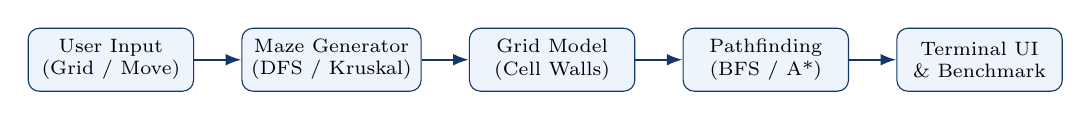
\begin{tikzpicture}[
node distance=6mm,
box/.style={rectangle,rounded corners,draw=GEUBlue,fill=GEULightBlue,
minimum width=2.1cm,minimum height=8mm,align=center,font=\scriptsize},
arrow/.style={-{Latex[length=2mm]},thick,draw=GEUBlue}
]
\node[box] (a) {User Input\\(Grid / Move)};
\node[box,right=of a] (b) {Maze Generator\\(DFS / Kruskal)};
\node[box,right=of b] (c) {Grid Model\\(Cell Walls)};
\node[box,right=of c] (d) {Pathfinding\\(BFS / A*)};
\node[box,right=of d] (e) {Terminal UI\\\& Benchmark};
\draw[arrow] (a)--(b); \draw[arrow] (b)--(c); \draw[arrow] (c)--(d); \draw[arrow] (d)--(e);
\end{tikzpicture}
\end{center}
\vspace{3mm}
\begin{columns}[T,totalwidth=\textwidth]
\column{.48\textwidth}
\textbf{\color{GEUBlue}Major Components}
\begin{itemize}\itemsep2pt
\item \texttt{Maze} \& \texttt{Cell}: Grid ownership and wall state.
\item \texttt{MazeGenerator}: Abstract generation strategy.
\item \texttt{MazeSolver}: Abstract pathfinding strategy.
\item \texttt{Player}: Movement \& collision detection.
\end{itemize}
\column{.48\textwidth}
\textbf{\color{GEUBlue}Data / Control Flow}
\begin{itemize}\itemsep2pt
\item User defines dimensions $\rightarrow$ Maze generated.
\item Player traverses grid via key commands.
\item Solvers evaluate grid as undirected graph.
\item Execution metrics output to terminal.
\end{itemize}
\end{columns}
\end{frame}

% 8: Technology Stack & Methodology
\begin{frame}{Technology Stack \& Methodology}
\begin{columns}[T,totalwidth=\textwidth]
\column{.48\textwidth}
\begin{block}{Technology Stack}
\begin{itemize}\itemsep2pt
\item \textbf{Language:} C++ (ISO C++17 Standard)
\item \textbf{Data Structures:} \texttt{std::vector}, \texttt{std::priority\_queue}, \texttt{std::stack}, Custom DSU
\item \textbf{Build Tool:} \texttt{g++} / CMake
\item \textbf{Version Control:} Git \& GitHub
\item \textbf{Optional Graphics:} SDL2 (Stretch Goal)
\end{itemize}
\end{block}
\column{.48\textwidth}
\begin{block}{Development Methodology}
\begin{enumerate}\itemsep2pt
\item Architecture \& Strategy Interface Design
\item Core Grid \& DFS Generation
\item Terminal Display \& Collision Engine
\item BFS \& A* Solver Implementation
\item Benchmarking \& Evaluation
\end{enumerate}
\end{block}
\end{columns}
\vfill
\begin{center}
\smallnote{Selected C++17 for zero-overhead abstractions and direct control over memory structures.}
\end{center}
\end{frame}

% 9: Initial Progress & Team Contribution
\begin{frame}{Initial Progress \& Team Contribution}
\begin{columns}[T,totalwidth=\textwidth]
\column{.40\textwidth}
\textbf{\color{GEUBlue}Progress Achieved (Phase-I)}
\begin{itemize}\itemsep3pt
\item System design \& UML architecture complete.
\item \texttt{Cell} and \texttt{Maze} models implemented.
\item Iterative DFS generator working.
\item Player movement and collision active.
\item BFS pathfinder with parent maps operational.
\end{itemize}
\column{.56\textwidth}
\textbf{\color{GEUBlue}Individual Contribution}
\vspace{2mm}
\scriptsize\renewcommand{\arraystretch}{1.3}
\begin{tabularx}{\textwidth}{@{}R{2.0cm}R{1.8cm}Y@{}}
\toprule
Member & Role & Contribution\\
\midrule
Tanmay Kumar & Lead / Arch & Grid Architecture, Interfaces, Execution Loop\\
Sparsh Saxena & Core Dev & Iterative DFS Generator, BFS Solver, A* Pathfinder\\
Hemang Sethi & Dev / UI & Player Movement, Collision Checks, Terminal UI, DSU\\
\bottomrule
\end{tabularx}
\end{columns}
\end{frame}

% 10: Roadmap, Expected Outcomes & References
\begin{frame}{Roadmap, Expected Outcomes \& References}
\setbeamerfont{itemize/enumerate body}{size=\footnotesize}
\begin{columns}[T,totalwidth=\textwidth]
\column{.31\textwidth}
\textbf{\color{GEUBlue}Roadmap}
\begin{enumerate}\itemsep3pt
\item \textbf{Phase-I:} System Design, DFS, BFS (Done)
\item \textbf{Phase-II:} A*, Kruskal's, Metrics (In Progress)
\item \textbf{Phase-III:} Comparative Analysis \& GUI Demo
\end{enumerate}
\column{.31\textwidth}
\textbf{\color{GEUBlue}Expected Outcomes}
\begin{itemize}\itemsep3pt
\item Fully functional C++ terminal application.
\item Measurable timing \& node traversal comparison.
\item Modular, extensible algorithm framework.
\end{itemize}
\column{.33\textwidth}
\textbf{\color{GEUBlue}References}
\begin{enumerate}\itemsep3pt
\item Cormen, T. H., et al. \textit{Introduction to Algorithms}. MIT Press.
\item Gamma, E., et al. \textit{Design Patterns}. Addison-Wesley.
\item ISO/IEC C++17 Standard Specifications.
\end{enumerate}
\end{columns}
\vfill
\begin{center}
\colorbox{GEUBlue}{\parbox{.50\textwidth}{\centering\color{white}\textbf{Thank You}\\Questions \& Suggestions}}
\end{center}
\end{frame}

\end{document}